\documentclass[letterpaper,addpoints,answers]{exam}
\usepackage{graphicx}
\usepackage{multicol}
\usepackage{wrapfig}
\usepackage{tikz}

\usetikzlibrary{calc}

\makeatletter
\def\grd@save@target#1{%
  \def\grd@target{#1}}
\def\grd@save@start#1{%
  \def\grd@start{#1}}
\tikzset{
  grid with coordinates/.style={
    to path={%
      \pgfextra{%
        \edef\grd@@target{(\tikztotarget)}%
        \tikz@scan@one@point\grd@save@target\grd@@target\relax
        \edef\grd@@start{(\tikztostart)}%
        \tikz@scan@one@point\grd@save@start\grd@@start\relax
        \draw[minor help lines] (\tikztostart) grid (\tikztotarget);
        \draw[major help lines] (\tikztostart) grid (\tikztotarget);
        \grd@start
        \pgfmathsetmacro{\grd@xa}{\the\pgf@x/1cm}
        \pgfmathsetmacro{\grd@ya}{\the\pgf@y/1cm}
        \grd@target
        \pgfmathsetmacro{\grd@xb}{\the\pgf@x/1cm}
        \pgfmathsetmacro{\grd@yb}{\the\pgf@y/1cm}
        \pgfmathsetmacro{\grd@xc}{\grd@xa + \pgfkeysvalueof{/tikz/grid with coordinates/major step x}}
        \pgfmathsetmacro{\grd@yc}{\grd@ya + \pgfkeysvalueof{/tikz/grid with coordinates/major step y}}
        \foreach \x in {\grd@xa,\grd@xc,...,\grd@xb}
        \node[anchor=north] at (\x,\grd@ya) {\pgfmathprintnumber{\x}};
        \foreach \y in {\grd@ya,\grd@yc,...,\grd@yb}
        \node[anchor=east] at (\grd@xa,\y) {\pgfmathprintnumber{\y}};
      }
    }
  },
  minor help lines/.style={
    help lines,
    gray,
    line cap =round,
    xstep=\pgfkeysvalueof{/tikz/grid with coordinates/minor step x},
    ystep=\pgfkeysvalueof{/tikz/grid with coordinates/minor step y}
  },
  major help lines/.style={
    help lines,
    line cap =round,
    line width=\pgfkeysvalueof{/tikz/grid with coordinates/major line width},
    xstep=\pgfkeysvalueof{/tikz/grid with coordinates/major step x},
    ystep=\pgfkeysvalueof{/tikz/grid with coordinates/major step y}
  },
  grid with coordinates/.cd,
  minor step x/.initial=.5,
  minor step y/.initial=.2,
  major step x/.initial=1,
  major step y/.initial=1,
  major line width/.initial=1pt,
}
\makeatother

\tikzset{
    right angle quadrant/.code={
        \pgfmathsetmacro\quadranta{{1,1,-1,-1}[#1-1]}     % Arrays for selecting quadrant
        \pgfmathsetmacro\quadrantb{{1,-1,-1,1}[#1-1]}},
    right angle quadrant=1, % Make sure it is set, even if not called explicitly
    right angle length/.code={\def\rightanglelength{#1}},   % Length of symbol
    right angle length=2ex, % Make sure it is set...
    right angle symbol/.style n args={3}{
        insert path={
            let \p0 = ($(#1)!(#3)!(#2)$) in     % Intersection
                let \p1 = ($(\p0)!\quadranta*\rightanglelength!(#3)$), % Point on base line
                \p2 = ($(\p0)!\quadrantb*\rightanglelength!(#2)$) in % Point on perpendicular line
                let \p3 = ($(\p1)+(\p2)-(\p0)$) in  % Corner point of symbol
            (\p1) -- (\p3) -- (\p2)
        }
    }
}

\begin{document}

\begin{coverpages}
 \large\bfseries
 
 \noindent 
 Physics 107: Physics for Life-Sciences

 \vspace{2ex}
 \noindent
 Midterm Exam: October 19, 2015

 \vspace{3ex}
 \noindent 
 This test is administered under the rules and regulations of the honor code of the College of William \& Mary.

 \vspace{2ex}
 \noindent 
 Name:\enspace\makebox[2.3in]{\hrulefill} \\

 \noindent 
 Signature:\enspace\makebox[2in]{\hrulefill} \\

 \vspace{5ex}
 \noindent 
 Instructions:
 \begin{itemize}
  \item This is a closed book, closed notes test.
  \item Calculators are NOT needed and NOT allowed. Devices with wireless connections are NOT allowed.
  \item Start your work from the fundamental equations on the formula sheet, and derive any additional expressions that you may need.
  \item Circle your answer for each part of each problem. 
  \item Clearly mark out any work that you wish the grader to disregard.  Do not waste your time erasing.
  \item Your work will be graded based on your ability to write down a logical and organized solution grounded in the correct assessment of the physics of a situation. No credit will be given for an answer that is not justified by a logical solution or where that justification is not organized or readable. Partial credit will be given up to the point where your solution departs from a correct analysis of the physics involved for any given part of a problem.
 \end{itemize}

 \pagebreak

 \begin{center}
  \gradetable[v][questions]
 \end{center}
 
\end{coverpages}
 

\begin{questions}

\printanswers

% 3 multiple choice questions

\begin{question}
A contestant $a$ in the winter games pushes a block of ice across a frozen lake with his arms at an angle of $25^\circ$ below the horizontal. A second contestant $b$ pulls an identical block of ice with a rope over his shoulder at an angle of $25^\circ$ above the horizontal. Both contestants are shown in the figure below.
\begin{center}
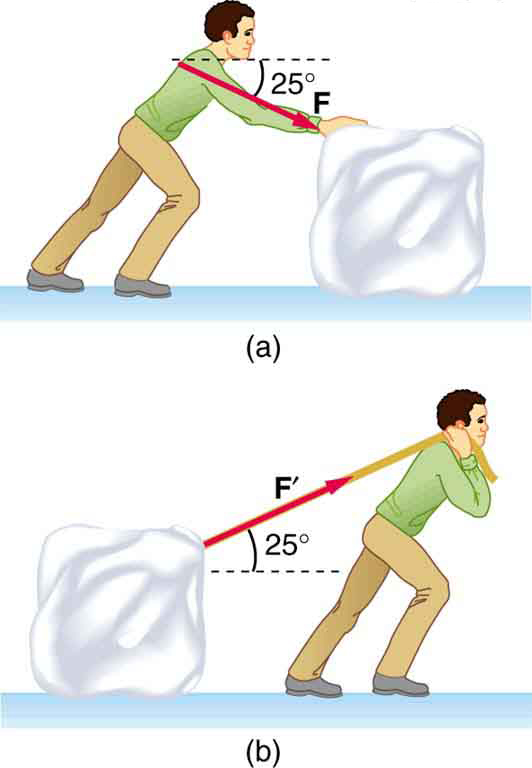
\includegraphics[width=0.3\textwidth]{test2/block_on_ice}
\end{center}
\begin{parts}
\part[5] Which contestant must exert a larger force $F$ to move the block with a constant velocity?
\begin{checkboxes}
 \correctchoice Contestant $a$ has to exert a larger force.
 \choice Contestant $b$ has to exert a larger force.
 \choice Both contestants have to exert the same force.
 \choice Unable to determine without additional information.
\end{checkboxes}
\part[5] Explain in words the reason for your answer above.
\begin{solution}[1in]
Since the contestant $a$ pushes down on the block, the normal force $N$ will be larger. This will result in a larger force of kinetic friction $f_k$ resisting the motion. That, in turn, will require a larger force $F$ to overcome.
\end{solution}
\end{parts}
\end{question}

\begin{question}[5]
An object moves in a circular path at a constant speed. Compare the direction of the object's velocity and acceleration vectors.
\begin{checkboxes}
 \choice Both vectors point in the same direction.
 \choice The vectors point in opposite directions.
 \correctchoice The vectors are perpendicular to each other.
 \choice The question is meaningless since one of the vectors is zero.
 \choice The question is meaningless since the relative orientation of the two vectors will change.
\end{checkboxes}
\end{question}

\begin{question}[5]
Two marbles, one twice as heavy as the other, are dropped from rest to the ground from the roof of a building. Ignore any air resistance. Just before hitting the ground, the heavier marble has a kinetic energy that is\ldots
\begin{checkboxes}
 \choice \ldots equal to the kinetic energy of the lighter marble.
 \correctchoice \ldots twice the kinetic energy of the lighter marble.
 \choice \ldots half of the kinetic energy of the lighter marble.
 \choice \ldots four times the kinetic energy of the lighter marble.
 \choice \ldots impossible to determine without additional information.
\end{checkboxes}
\end{question}

\pagebreak

% question 1

\begin{question}
A rotating space station is said to create \emph{artificial gravity} -- a loosely-defined term used for an acceleration that would be crudely similar to gravity. The outer wall of the rotating space station would become a floor for the astronauts, and centripetal acceleration supplied by the floor would allow astronauts to exercise and maintain muscle and bone strength more naturally than in non-rotating space environments. An example of such a setup is \emph{Space Station V} from the movie \emph{2001: A Space Odyssey} as shown below.
\begin{center}
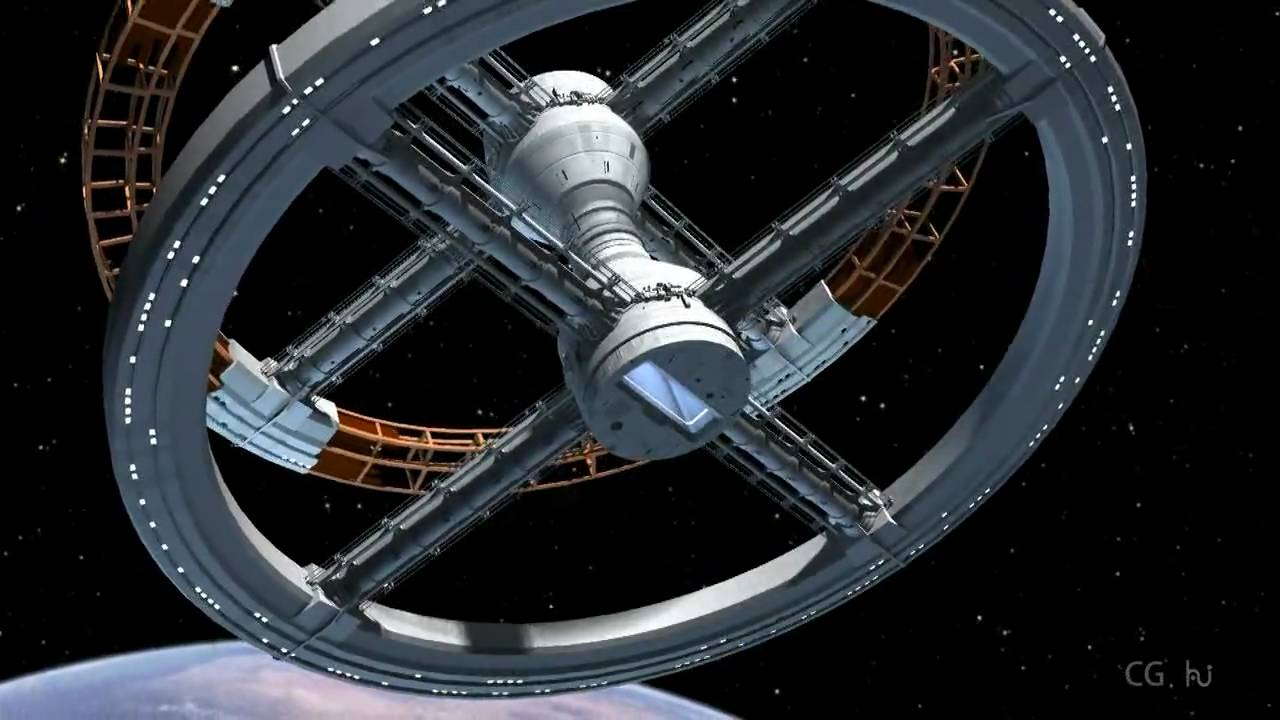
\includegraphics[height=0.16\textheight]{test2/2001-space-station-V} 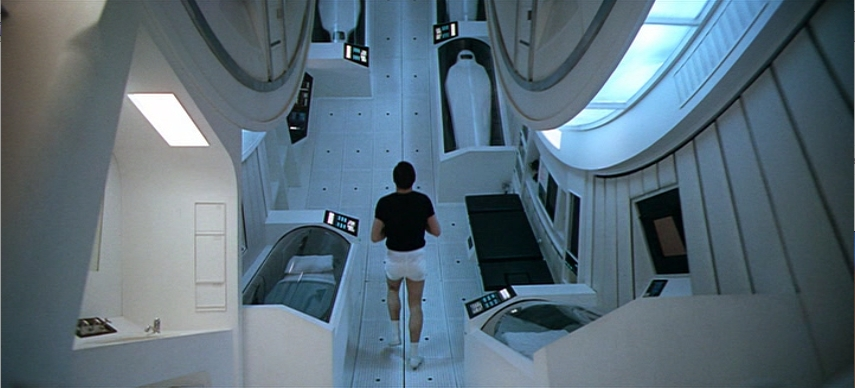
\includegraphics[height=0.16\textheight]{test2/2001-discovery-interior}
\end{center}
\begin{parts}
\part[5] If the space station is 500\,m in diameter, what angular velocity (in radians per second) would produce an artificial gravity similar to that on Earth inside the outer wall of the station? You may approximate the magnitude of the Earth's gravitational acceleration $g$ as $10.0\,\mbox{m}/\mbox{s}^2$.
\begin{solution}[1in]
The centripetal acceleration $a_c = r\omega^2$ must be numerically equal to the gravitational acceleration $g$. This means that the angular velocity $\omega$ must be $\omega = \sqrt{g/r} = \sqrt{0.04} = 0.2$\,rad/s.
\end{solution}
\part[5] What is the period of revolution of the space station? You may use $2\pi \approx 6.4$.
\begin{solution}[1in]
With $T = 2\pi/\omega$ we find $T = 32$\,s.
\end{solution}
\part[5] An astronaut standing inside the space station drops a ball to the floor. Describe the motion of the ball as seen by a non-rotating observer outside the space station. What will be the acceleration of the ball for that outside observer?
\begin{solution}[2in]
On the space station the centripetal acceleration points to the center of rotation, \emph{i.e.} upwards in the frame of reference of the astronauts, and is felt by all objects participating in the uniform circular motion. The ball is not acted upon by any force so it does not experience any acceleration and must describe a straight line to the outside observer.
\end{solution}
\end{parts}
\end{question}

\pagebreak

% question 2

\begin{question}
The spring driven ball launcher in a pinball machine launches a 100\,g metal ball by compressing the spring by 10\,cm. The pinball machine's surface is tilted at an angle of 30$^\circ$ with the horizontal. We want to determine the spring constant $k$ such that we can launch the ball and reach the highest point A, a distance of 1\,m away from C, as measured along the tilted playing surface. Assume that frictional effects are negligible. You may approximate the magnitude of the gravitational acceleration $g$ as $10.0\,\mbox{m}/\mbox{s}^2$.

\begin{center}
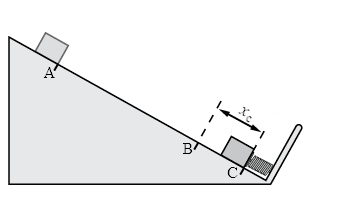
\includegraphics[width=0.3\textwidth]{test2/pinball}
\end{center}

\begin{parts}
\part[5] What is the mechanical energy (kinetic and potential energy) when the ball reaches the highest point A and is momentarily stationary there?
\begin{solution}[1.25in]
When the ball reaches the highest point it is instantaneously at rest, so the kinetic energy is zero. The mechanical energy is then $KE_A + PE_A = m g |AC| \sin 30^\circ = 0.5$\,J.
\end{solution}
\part[5] What is the mechanical energy (kinetic and potential energy) when the spring in the launcher is fully compressed at point C, immediately before launching the ball?
\begin{solution}[1.25in]
The mechanical energy when the spring is compressed is $KE_C + PE_C = 0 + \frac{1}{2} k x_C^2$. This must be equal to 0.5\,J as well. When the ball is released, the mechanical energy is $KE_B + PE_B = \frac{1}{2} m v^2 + m g x_C \sin 30^\circ$. 
\end{solution}
\part[5] What is the value for the spring constant $k$ such that the ball reaches the highest point A?
\begin{solution}[1.25in]
Since $\frac{1}{2} k x_C^2 = 0.5$\,J, this means that $k = 2 (0.5\,\mbox{J})/x_C^2$, or $k = 100\,\mbox{N}/\mbox{m} = 1\,\mbox{N}/\mbox{cm}$.
\end{solution}
\part[5] What is the speed of the ball as it leaves the launcher at point B?
\begin{solution}[1.5in]
The kinetic energy at point B is 0.5\,J minus $m g |BC| \sin 30^\circ = 0.05$\,J, or 0.45\,J. Since this is equal to the kinetic energy $\frac{1}{2} m v^2$ the speed must be $v^2 = 2 (0.45\,\mbox{J})/m$ or $v = 3$\,m/s.
\end{solution}
\end{parts}
\end{question}

\pagebreak

% question 3

\begin{question}
You have been hired by the W\&M Police Department to examine their new pistols. They have asked you to determine the velocity of the bullets when they leave the handgun. To test this you fire a standard $m_1 = 2.0$\,g bullet toward a wooden block hanging from a rope (called a \emph{ballistic pendulum}). When the bullet hits the block is embeds itself in the wood. You observe that the block swings upward after the collision. When you do your experiment you note that the block swings to a height of $h = 0.20$\,m above its original hanging position. You measure the mass $m_1 + m_2$ of the block with the bullet embedded to be exactly 1.000\,kg. You may approximate the magnitude of the gravitational acceleration $g$ as $10.0\,\mbox{m}/\mbox{s}^2$.
\begin{center}
 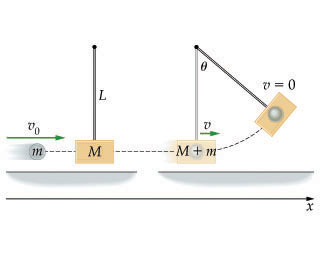
\includegraphics[width=0.6\textwidth]{test2/ballistic_pendulum}
\end{center}

\begin{parts}
 \part[5] What is the potential energy of the block and bullet when it is at its highest position?
 \begin{solution}[1.25in]
 The potential energy at the highest point is given by $PE = m g h$, with mass $m = m_1 + m_2$ of the bullet and the wooden block. This results in $PE = (m_1 + m_2) g h = 2.000$\,J.
 \end{solution}
 \part[5] What is the speed of the block just after the bullet hits the block?
 \begin{solution}[1.25in]
 The total mechanical energy (sum of potential energy and kinetic energy) immediately after the collision must be equal to the total mechanical energy at the highest position. This means that $\frac{1}{2} (m_1 + m_2) v^2 = (m_1 + m_2) g h$. The speed immediately after the collision must therefore be $v = \sqrt{2 g h} = 2.0$\,m/s.
 \end{solution}
 \part[5] What is the speed of the bullet before the collision?
 \begin{solution}[1.5in]
 Conservation of momentum relates the speed of the bullet $v_1$ and the speed of the block $v_2$ before the collision with the speed $v$ after the collision (and found in the previous part): $m_1 v_1 + m_2 v_2 = (m_1 + m_2) v$. Because the block is initially at rest, $v_2 = 0$, this results in an expression for $v_1$,
 \begin{equation}
 v_1 = \frac{m_1 + m_2}{m_1} v = \frac{1.000\,\mbox{kg}}{0.0002\,\mbox{kg}} (2.0\,\mbox{m}/\mbox{s}) = 1000\,\mbox{m}/\mbox{s}.
 \end{equation}
 \end{solution}
 \part[5] How much energy is converted into other energies (\emph{e.g.} heat) in this inelastic collision?
 \begin{solution}[1.5in]
 The initial kinetic energy of the bullet is $\frac{1}{2} m_1 v_1^2 = 1000$\,J. This means that 998\,J is converted in heat.
 \end{solution}
 \end{parts}
\end{question}

\end{questions}

 \pagebreak
 
 {\Large Possibly useful relations (feel free to detach this page):}
  
%  \fontseries{\seriesdefault}
%  \begin{multicols}{2}
%  \Large
%  \noindent
%  $\vec{v}_{avg} = \Delta\vec{x} / \Delta t$ \\
%  $x = x_0 + v_0 t + \frac{1}{2} a t^2$ \\
%  $v^2 = v_0^2 + 2 a (x - x_0)$ \\
%  $R = \frac{v_0^2}{g}\sin 2\theta$ \\
%  $\vec{F}_{net} = m \vec{a}$ \\
%  $\vec{W} = m \vec{g}$ \\
%  $\cos\theta = \hbox{adjacent}/\hbox{hypotenuse}$ \\
%  $\sin\theta = \hbox{opposite}/\hbox{hypotenuse}$ \\
%  $\sin 30^\circ = \cos 60^\circ = \frac{1}{2}$ \\
%  $\cos 30^\circ = \sin 60^\circ = \frac{\sqrt{3}}{2}$ \\
 
%  \noindent
%  $\vec{a}_{avg} = \Delta\vec{v} / \Delta t$ \\
%  $v = v_0 + a t$ \\
%  $v_{avg} = \frac{v_0 + v}{2}$ \\
%  $h = \frac{v_0^2}{2 g} \sin^2 \theta$ \\
%  $\vec{F}_{BA} = - \vec{F}_{AB}$ \\
%  $\vec{g} = 9.80\,m/s^2$ downward \\
%  $x = \frac{-b \pm \sqrt{b^2 - 4 a c}}{2 a}$ \\
%  $\tan\theta = \sin\theta / \cos\theta$ \\
%  $\tan 45^\circ = 1$ \\
%  \end{multicols}

 \fontseries{\seriesdefault}
 \begin{multicols}{2}
 \Large
 \noindent
 $\vec{v}_{avg} = \Delta\vec{x} / \Delta t$ \\
 $\vec{a}_{avg} = \Delta\vec{v} / \Delta t$ \\
 $x = x_0 + v_0 t + \frac{1}{2} a t^2$ \\
 $v = v_0 + a t$ \\
 $v_{avg} = \frac{v_0 + v}{2}$ \\
 $v^2 = v_0^2 + 2 a (x - x_0)$ \\
 $\vec{F}_{net} = m \vec{a}$ \\
 $\vec{F}_{BA} = - \vec{F}_{AB}$ \\
 $W = F d \cos\theta$ \\
 $W_{net} = -\Delta PE = \Delta KE$ \\
 $KE = \frac{1}{2} m v^2$ \\
 $PE_k = \frac{1}{2} k x^2$ \\
 $PE_g = m g h$ \\
 $KE_i + PE_i + W_{nc} = KE_f + PE_f$ \\
 $P = \frac{W}{\Delta t}$ \\
 $\hbox{Eff} = \frac{W_{out}}{E_{in}}$ \\
 $\cos\theta = \hbox{adjacent}/\hbox{hypotenuse}$ \\
 $\sin\theta = \hbox{opposite}/\hbox{hypotenuse}$ \\
 $\tan\theta = \sin\theta / \cos\theta$ \\
 $\sin 30^\circ = \cos 60^\circ = \frac{1}{2}$ \\
 $\cos 30^\circ = \sin 60^\circ = \frac{\sqrt{3}}{2}$ \\
 $\tan 45^\circ = 1$ \\

 \noindent
 $R = \frac{v_0^2}{g}\sin 2\theta$ \\
 $h = \frac{v_0^2}{2 g} \sin^2 \theta$ \\
 $0 \le f_s \le \mu_s N$ \\
 $f_k = \mu_k N$ \\
 $\frac{F}{A} = Y \frac{\Delta L}{L}$ \\
 $F_k = -k x$ \\
 $\vec{W} = m \vec{g}$ \\
 $\vec{g} = 9.80\,\mbox{m}/\mbox{s}^2$ downward \\
 $F_G = G \frac{m M}{r^2}$ \\
 $G = 6.67 \times 10^{-11}\,\mbox{N}\cdot\mbox{m}^2/\mbox{kg}^2$ \\
 $\vec{I} = \vec{F}_{avg} \Delta t$ \\
 $\vec{p} = m \vec{v}$ \\
 $\vec{F}_{net} = \frac{\Delta \vec{p}}{\Delta t}$ \\
 $v_1 - v_2 = v'_2 - v'_1$ \\
 $\theta = \frac{s}{r}$ \\
 $v = r \omega$ \\
 $f = \frac{1}{T}$ and $\omega = 2 \pi f = \frac{2 \pi}{T}$ \\
 $a_c = \frac{v^2}{r} = r \omega^2$ \\
 $F_c = m\frac{v^2}{r} = m r \omega^2$ \\
 $1\,\hbox{cal} = 4.186$\,J and $1\,\hbox{Cal} = 1000$\,cal \\ 
 $x = \frac{-b \pm \sqrt{b^2 - 4 a c}}{2 a}$ \\
 \end{multicols}

\end{document}
